\documentclass[11pt]{article}
\usepackage{epsfig}    % to insert postscript figures
\begin{document}

\title{Estimating $\mathcal{R}_t$ from Covid-19 case counts}
\author{ Hugh Murrell, Dan Murrell and Ben Murrell}
\maketitle

\begin{abstract}
Here we give an interpretation of
the {\it effective reproduction number}, $\mathcal{R}_t$ that arises
from the Susceptible-Infectious (SI) model 
for the spread of infectious disease. We also outline a simple scheme for
estimating $\mathcal{R}_t$ from daily case counts.
\end{abstract}

\section{The standard SI model}
The Susceptible-Infectious (SI) model \cite{Wikipedia} is often used 
to study the spread of infectious disease by tracking the number ($S$) of people 
susceptible to the disease and the number ($I$) of people infectious with the disease.

Based on the model, the only way that a person can leave the susceptible
group is to be infected and become immediately infectious, and the only way 
that a person can leave the infectious group is to recover or die. 
It is further assumed that those who have recovered or died from the disease 
are no longer susceptible.

It is also assumed that all those who have not had the disease are 
equally susceptible and that the probability of their contracting the 
disease at time $t+1$ is proportional to the product of $S$ and $I$ at time $t$. 

These assumptions lead us to a pair of difference equations
for $S$ and $I$, where the unit of time $t$ is one day:

\begin{eqnarray}
S_{t+1} & = & S_t - \beta \frac{S_t I_t}{N} \label{eq1a} \\
I_{t+1} & = & I_t + \beta \frac{S_t I_t}{N} - \gamma I_t \label{eq1b} 
\end{eqnarray}

Here the parameter $\beta \geq 0$ controls the rate at which the susceptible
become infected and the parameter $\gamma \geq 0$ controls the rate
at which the infectious recover or die. The parameter $N$ is the size of
the {\bf initial} susceptible population and is usually assumed constant. 
The number of infected persons who are no longer infectious
is given by $N-(S_t+I_t)$.

The susceptible time series ($S$) is a monotonically decreasing sequence
starting at $S_0 = N$ just before the outbreak of the disease whilst the infectious 
group $I$ starts at $I_0 = 0$ just before the outbreak but then climbs and falls
depending on interventions but eventually dies out to zero when
the disease has run its course. 

With this model the trajectories of $S_t$ and $I_t$ are pre-determined at the outset by
the parameters, $\beta$, $\gamma$ and $N$. See Figure \ref{fig1} for an
example trajectory.

\begin{figure}[ht]
\begin{center}
  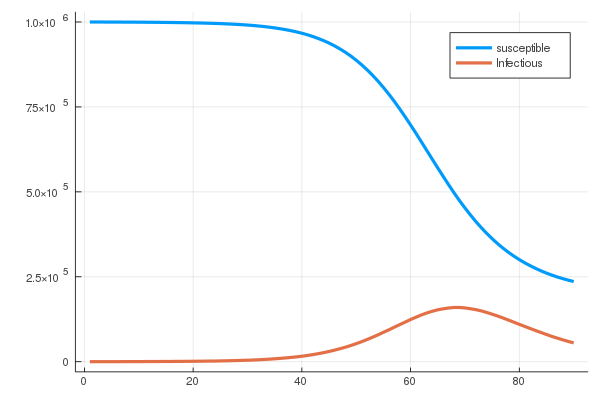
\epsfig{file=RtSIM.png,height=2in}
\end{center}
\caption{Susceptible and Infectious time series
for user defined parameters, $\gamma = \frac{1}{7}$, $N=10^6$ and $\beta = 2 \frac{\gamma}{N}$.
}  
\label{fig1}
\end{figure}

\section{Introducing $\mathcal{R}_t$}

To gain some {\it control} over an epidemic, authorities can enforce quarantine or
social distancing measures which may affect some of the model parameters.
The parameter $\gamma$ cannot be manipulated through such measures
as it is the reciprocal of the length of the infectious period which in the case of
Covid-19 is estimated to be about one week, so $\gamma = \frac{1}{7}$.

The other two parameters, $\beta$ and $N$, can be manipulated via interventions
and it is a common practice to define a quantity called the {\it effective} reproduction number, 
$\mathcal{R}_t$ as follows:

\begin{eqnarray}
\mathcal{R}_{t} & = & \frac{\beta}{\gamma}\frac{S_t}{N} \label{eq2} 
\end{eqnarray}

and then recast the discrete SI model as:

\begin{eqnarray}
S_{t+1} & = & S_t - \gamma \mathcal{R}_t  I_t \label{eq3a} \\
I_{t+1} & = & I_t +\gamma  I_t ( \mathcal{R}_t - 1 ) \label{eq3b} 
\end{eqnarray}

Note that $ \mathcal{R}_0 = \frac{\beta}{\gamma} $
which is called the {\bf basic} reproduction number and tells us how many
persons an infected person will infect during their infectious period at the
start of an epidemic and before any interventions can be mounted.
In the case depicted in figure \ref{fig1}, the basic reproduction number is
$\mathcal{R}_0 = \frac{\beta}{\gamma} S_0 = 2 $.

Note that if no interventions are put in place during the course of the epidemic 
then $\mathcal{R}_t$ will decrease monotonically as $S_t$ decreases.
The goal of interventions is to decrease $\mathcal{R}_t$ faster than
its natural decline induced by the diminishing pool of susceptible persons.
In particular it is desirable to force $\mathcal{R}_t < 1$ so that 
the pool of infectious is smaller when a person leaves the pool
than when he enters it. 

To see if an intervention is successful or not we must have some
way of estimating the current value of $\mathcal{R}_t$ from 
case counts.

\section{Estimating $\mathcal{R}_t$ from case count data}

An estimate for yesterday's $\mathcal{R}_t$ value can be obtained
by comparing the size of yesterday's infectious pool with the size
of today's infectious pool by rewriting equation \ref{eq3b} as follows.

\begin{eqnarray}
\mathcal{R}_t  & =  & 1 + \frac{1}{\gamma}  \left( \frac{ I_{t+1} - I_t} {I_t }  \right) \label{eq4b} 
\end{eqnarray}

$\gamma \mathcal{R}_t \geq 0$ measures the likelihood
of transmitting the disease when an infected and a susceptible come
in contact.   Hence $\mathcal{R}_t$ is the number of transmissions
caused by an infected person during his infectious period.

From the figure, one can see that if $( \beta / k ) S(0)$ is much greater than $1$,
then the entire population quickly becomes infected and then recovered/dead.
For $( \beta / k ) S(0)$ less than $1$, the infection seems to die out after
only a small percentage of the population has been infected.  For values
somewhat greater than $1$, the number infected and hence later recovered/dead
seems to be a larger fraction but not necessarily all of the population.
The Matlab code used to produce these plots can be found in Appendix A.

\section{Conclusions}
The results of this simple model look fairly reasonable and so they might be
used to decide on a strategy for curtailing an epidemic through vaccinations,
quarantines, etc.  Many enhancements to the model can be made.  For a discussion 
of some of these, see, for example, \cite{Wikipedia}.  

\newpage
\appendix
\section{Matlab Code for Producing Plots}

\begin{verbatim}
global betaglob  % Global variables to be supplied to function sirdot.
global kglob     % Give them funny names so they won't be used elsewhere.

kglob = 0.1;               % Set k.
betas = [.005; .0005; .0002; .0001];
for kase=1:4,
  betaglob = betas(kase);  % Set beta.
  tfinal = 50;  if kase > 2, tfinal = 500; end;
  [tout,sout] = ode45('sirdot',[0 tfinal], [990; 10; 0]); % Solve with ode45.

  subplot(2,2,kase)  
  plot(tout,sout(:,1),'-', tout,sout(:,2),'--', tout,sout(:,3),'-.');
  xlabel('t'), ylabel('population')
  if kase==1,
    title('beta = 0.005, k = 0.1, (beta/k)*S0 = 49.5');
  elseif kase==2,
    title('beta = 0.0005, k = 0.1, (beta/k)*S0 = 4.95');
  elseif kase==3,
    title('beta = 0.0002, k = 0.1, (beta/k)*S0 = 1.98');
  else
    title('beta = 0.00005, k = 0.1, (beta/k)*S0 = 0.495');
  end;
end;

function sirprime = sirdot(t,sir)
global betaglob
global kglob
beta = betaglob;  k = kglob;

sirprime(1,1) = -beta*sir(1)*sir(2);
sirprime(2,1) = beta*sir(1)*sir(2) - k*sir(2);
sirprime(3,1) = k*sir(2);
\end{verbatim}

\newpage

\begin{thebibliography}{99}

\bibitem{Johnson}  Johnson, Teri, {\em Mathematical Modeling of Diseases:
Susceptible-Infected-Recovered (SIR) Model}, Math 4901 Senior Seminar, 
University of Minnesota, Spring 2009.
\verb+http://www.morris.umn.edu/academic/math/Ma4901/Sp09/Final/Teri-Johnson-Final.pdf+ .

\bibitem{Tung} Tung, K.~K., {\em Topics in Mathematical Modeling},
Princeton University Press, 2007.

\bibitem{Wikipedia} Wikipedia, {\em Compartmental models in epidemiology},
\verb+http://en.wikipedia.org/wiki/Compartmental_models_in_epidemiology+ .

\end{thebibliography}
\end{document}


